\documentclass{article}
\usepackage[dvipsnames]{xcolor} % Required for specifying custom colors
\usepackage[showframe=false]{geometry} % Required for adjusting page dimensions and margins

% Packages for custom shapes and boxes
\usepackage{tikz} % Required for drawing custom shapes
\usepackage[framemethod=TikZ]{mdframed} % Required for creating the theorem, definition, exercise and corollary boxes
% \newcounter{theo}[section]\setcounter{theo}{0}

% THEOREM BOXES
\newcounter{theo}[section]\setcounter{theo}{0}
\renewcommand{\thetheo}{\arabic{section}.\arabic{theo}}

\newenvironment{theo}[2][]{%
    \refstepcounter{theo}

    \ifstrempty{#1}%
    % if condition (without title)
    {\mdfsetup{%
            frametitle={%
                    \tikz[baseline=(current bounding box.east),outer sep=0pt]
                    \node[anchor=east,rectangle,fill=black,text=white]
                    {\strut Theorem~\thetheo};}
        }%
        % else condition (with title)
    }{\mdfsetup{%
            frametitle={%
                    \tikz[baseline=(current bounding box.east),outer sep=0pt]
                    \node[anchor=east,rectangle,fill=black,text=white]
                    {\strut Theorem~\thetheo:~#1};}%
        }%
    }%
    % Both conditions
    \mdfsetup{%
        innertopmargin=6pt,innerbottommargin=12pt,linecolor=black,%
        linewidth=2pt,topline=true,%
        frametitleaboveskip=\dimexpr-\ht\strutbox\relax%
    }

    \begin{mdframed}[]\relax}{%
    \end{mdframed}}

% DEFINITION BOXES
\newcounter{Def}[section]\setcounter{Def}{0}
\renewcommand{\theDef}{\arabic{section}.\arabic{Def}}

\newenvironment{Def}[2][]{%
    \refstepcounter{Def}

    \ifstrempty{#1}%
    % if condition (without title)
    {\mdfsetup{%
            frametitle={%
                    \tikz[baseline=(current bounding box.east),outer sep=0pt]
                    \node[anchor=east,rectangle,fill=black,text=white]
                    {\strut Definition~\theDef};}
        }%
        % else condition (with title)
    }{\mdfsetup{%
            frametitle={%
                    \tikz[baseline=(current bounding box.east),outer sep=0pt]
                    \node[anchor=east,rectangle,fill=black,text=white]
                    {\strut Definition~\theDef:~#1};}%
        }%
    }%
    % Both conditions
    \mdfsetup{%
        innertopmargin=6pt,
        innerbottommargin=12pt,
        linecolor=black,%
        linewidth=2pt,topline=true,%
        frametitleaboveskip=\dimexpr-\ht\strutbox\relax%
    }

    \begin{mdframed}[]\relax}{%
    \end{mdframed}}


% TIP BOXES
\newcounter{Tip}[section]\setcounter{Tip}{0}
\renewcommand{\theTip}{\arabic{section}.\arabic{Tip}}

\newenvironment{Tip}{%
    \refstepcounter{Tip}
    \mdfsetup{%
        backgroundcolor=OliveGreen!10,
        innertopmargin=12pt,
        innerbottommargin=0.5pt,
        linecolor=black,
        linewidth=0pt,
        topline=false,
        frametitleaboveskip=\dimexpr-\ht\strutbox\relax
    }
    \begin{mdframed}[]\relax
        \textbf{Tip:}
        }{%
    \end{mdframed}
}

% GREEN BOXES
\newenvironment{greenbox}{%
    \mdfsetup{%
        backgroundcolor=OliveGreen!10,
        innertopmargin=12pt,
        innerbottommargin=12pt,
        linecolor=black,
        linewidth=0pt,
        topline=false,
        frametitleaboveskip=\dimexpr-\ht\strutbox\relax
    }
    \begin{mdframed}[]\relax

        }{%
    \end{mdframed}
}

% GRAY BOXES
\newenvironment{graybox}{%
    \mdfsetup{%
        backgroundcolor=black!10,
        innertopmargin=12pt,
        innerbottommargin=12pt,
        linecolor=black,
        linewidth=0pt,
        topline=false,
        frametitleaboveskip=\dimexpr-\ht\strutbox\relax
    }
    \begin{mdframed}[]\relax

        }{%
    \end{mdframed}
}

% NOTE BOXES
\newcounter{Note}[section]\setcounter{Note}{0}
\renewcommand{\theNote}{\arabic{section}.\arabic{Note}}

\newenvironment{Note}{%
    \refstepcounter{Note}
    \mdfsetup{%
        backgroundcolor=black!10,
        innertopmargin=10pt,
        innerbottommargin=6pt,
        linecolor=black,
        linewidth=0pt,
        topline=false,
        frametitleaboveskip=\dimexpr-\ht\strutbox\relax
    }
    \begin{mdframed}[]\relax
        }{%
    \end{mdframed}
}

% GENERIC BOXES

\newenvironment{gbox}{%
    \mdfsetup{%
        backgroundcolor=white,
        innertopmargin=12pt,
        innerbottommargin=6pt,
        linecolor=black,
        linewidth=1pt,
        topline=true,
        frametitleaboveskip=\dimexpr-\ht\strutbox\relax
    }
    \begin{mdframed}[]\relax
        % Your content goes here
        }{%
    \end{mdframed}
}
 % This file contains the code for the boxes

% Packages for math symbols and images
\usepackage{amssymb} % Math symbols such as \mathbb
\usepackage{amsmath} % Required for \begin{align}...\end{align}
\usepackage{graphicx} % Required for including images

% Tables
\usepackage{multirow} % Required for creating multirow cells in tables
\usepackage{array} % Required for creating tables
\usepackage{colortbl} % Add this line to import the colortbl package
\setlength{\tabcolsep}{18pt} % Default value: 6pt
\renewcommand{\arraystretch}{1.5} % Default value: 1
\usepackage{changepage} % Required for adjusting the width of the table


% Package for customizing captions
\usepackage{caption}  % Required for customizing captions

\usepackage{setspace} % Required for adjusting line spacing

% commands

% Tikz
\tikzset{
    pics/machine/.style={
            code={
                    \coordinate (-in) at ({-0.5*\pgfkeysvalueof{/tikz/machine/width}},0);
                    \coordinate (-out) at ({0.5*\pgfkeysvalueof{/tikz/machine/width}},0);
                    \coordinate (-north) at (0,{0.5*\pgfkeysvalueof{/tikz/machine/height}});
                    \coordinate (-south) at (0,{-0.5*\pgfkeysvalueof{/tikz/machine/height}});
                    \path[/tikz/machine/filling]
                    ([shift={(-0.75em,0.5em)}]-in)
                    -- ([shift={(0,0.25em)}]-in)
                    -- ([shift={(0,-5pt)}]-north -| -in)
                    arc[start angle=180, end angle=90, radius=5pt]
                    -- ([shift={(-5pt,0)}]-north -| -out)
                    arc[start angle=90, end angle=0, radius=5pt]
                    -- ([shift={(0,0.25em)}]-out)
                    -- ([shift={(0.75em,0.5em)}]-out)
                    -- ([shift={(0.75em,-0.5em)}]-out)
                    -- ([shift={(0,-0.25em)}]-out)
                    -- ([shift={(0,5pt)}]-south -| -out)
                    arc[start angle=360, end angle=270, radius=5pt]
                    -- ([shift={(5pt,0)}]-south -| -in)
                    arc[start angle=270, end angle=180, radius=5pt]
                    -- ([shift={(0,-0.25em)}]-in)
                    -- ([shift={(-0.75em,-0.5em)}]-in)
                    -- cycle;
                    \draw[/tikz/machine/border]
                    ([shift={(-0.75em,0.5em)}]-in)
                    -- ([shift={(0,0.25em)}]-in)
                    -- ([shift={(0,-5pt)}]-north -| -in)
                    arc[start angle=180, end angle=90, radius=5pt]
                    -- ([shift={(-5pt,0)}]-north -| -out)
                    arc[start angle=90, end angle=0, radius=5pt]
                    -- ([shift={(0,0.25em)}]-out)
                    -- ([shift={(0.75em,0.5em)}]-out);
                    \draw[/tikz/machine/border]
                    ([shift={(0.75em,-0.5em)}]-out)
                    -- ([shift={(0,-0.25em)}]-out)
                    -- ([shift={(0,5pt)}]-south -| -out)
                    arc[start angle=360, end angle=270, radius=5pt]
                    -- ([shift={(5pt,0)}]-south -| -in)
                    arc[start angle=270, end angle=180, radius=5pt]
                    -- ([shift={(0,-0.25em)}]-in)
                    -- ([shift={(-0.75em,-0.5em)}]-in);
                    \node (-node) at (0,0) {#1};
                }
        },
    machine/width/.initial={10.5em},
    machine/height/.initial={5em},
    machine/filling/.style={
            left color=cyan!50!OliveGreen!25,
            right color=cyan!50!OliveGreen!25,
            middle color=cyan!50!OliveGreen!10
        },
    machine/border/.style={
            OliveGreen!50!cyan
        }
}

\newcommand{\Div}{%
    \par\noindent\hrulefill\par
}

\title{Not so Discrete Math}
\author{Christian Rudder}
\date{August 2024}

\begin{document}

\maketitle

\tableofcontents

% Intentionally left blank
\newpage
\thispagestyle{empty}
\mbox{}
\vfill
\begin{center}
    \textit{This page is left intentionally blank.}
\end{center}
\vfill
\newpage

\section{Sets}
\textbf{Opening Question:} What do we call a collection of things?
does order or repetition matter? Can we contain collection of other collections? Is an empty collection
considered a collection? How do we count members of a collection, and how do we define them?\\

\subsection{Introduction to Sets}
\hspace*{1em}
In discrete math we work with some group of `things,' a thing or something
we fancily call an \textbf{object}. A group or categorization of objects is called a set.

\begin{theo}[Set]{thm:set}
    Is a collection of objects.
\end{theo}

\noindent
\textbf{For Example:}
\begin{itemize}
    \item $S$ = The set of all students in a classroom.
    \item $A$ = The set of all vowels in the English alphabet.
    \item $\mathbb{Z}$ = The set of all integers.

\end{itemize}
Objects in a \textbf{set} are called \textbf{elements}.

\begin{theo}[Element]{thm:element}
    An object that is a member of a given set.
\end{theo}

\noindent
To expand on the previous example:
\begin{itemize}
    \item $S = \{s_1, s_2, s_3\}$, where $s_1, s_2, s_3$ are students, elements of the set.
    \item $A = \{a, e, i, o, u\}$, where $a, e, i, o, u$ are elements.
    \item $\mathbb{Z} = \{\ldots, -3, -2, -1, 0, 1, 2, 3, \ldots\}$, elements of integer set.
\end{itemize}
Curly braces denote a set, commas to separate elements,
The `$...$' or `ellipse' indicate that the set continues indefinitely in that direction.
When the set's pattern is clear to the reader, we use the dotted notation.\\

\noindent
Symbols used to denote members of a set:
\begin{itemize}
    \item `$\in$' = in the set.
    \item `$\notin$' = not in the set.
\end{itemize}

\begin{theo}[Membership]{thm:membership}
    If $x$ is an element of set $A$, $x \in A$.
    If $x$ is not an element of set $A$, $x \notin A$.
\end{theo}

\noindent
\textbf{For Example:} Given $A = \{a, e, i, o, u\}$,\\
$a \in A$, ``$a$ is an element of $A$,'' and
$b \notin A$, ``$b$ is not an element of $A$.''\\

\noindent
\textbf{Order nor repetition matter:}
\begin{itemize}
    \item $A = \{1, 2, 3\} = \{3, 2, 1\} = \{1, 2, 3, 3, 3, 3, 3\}$.
    \item $B = \{a, b, c\} = \{a, b, c, a, b, c\}$.
\end{itemize}

\begin{theo}[Properties of a Set]{thm:set_props}
    \begin{itemize}
        \item The order of elements does not matter.
        \item Duplicate elements are not counted.
    \end{itemize}
\end{theo}

\noindent
A subset is a set contained within another set. If the set $B$ is a subset of set $A$,
then every element in $B$ is also in $A$ as shown in Figure \ref{fig:subset}:


\begin{figure}[ht]
    \centering
    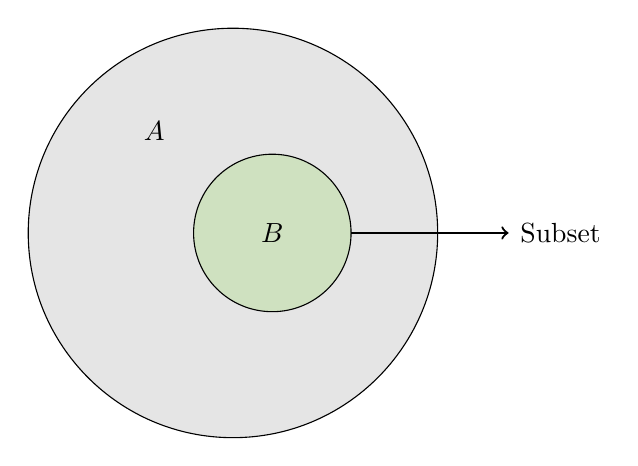
\begin{tikzpicture}
        % Set A
        \draw[fill=gray!20] (0,0) circle (2.6cm);
        \node at (-1,1.3) {$A$};

        % Set B
        \draw[fill=OliveGreen!20] (0.5,0) circle (1cm);
        \node at (0.5,0) {$B$};

        % Subset arrow
        \draw[->, thick] (1.5,0) -- (3.5,0);

        % Subset label
        \node at (4.16,0) {Subset};
    \end{tikzpicture}
    \caption{}
    \label{fig:subset}
\end{figure}


\noindent
Written $B \subseteq A$ or $A \supseteq B$, similar to the less than or
equal to signs `$\leq$' and `$\geq$'.

\begin{theo}[Subset]{thm:subset}
    If every element in set $B$ is also in set $A$, then $B$ is a subset of $A$.\\
    Denoted: $B \subseteq A$ or $A \supseteq B$.
\end{theo}

\noindent
\textbf{For Example:}
\begin{itemize}
    \item $\{-1, 0\} \subseteq \{-1, 0, 1, 2, 3\}$
    \item $\{-1, 1, 3\} \subseteq \{-1, 0, 1, 2, 3\}$
    \item $\{-1, 0, 1, 2, 3\} \subseteq \{-1, 0, 1, 2, 3\}$
    \item $\{-1, 7\} \not\subseteq \{-1, 0, 1, 2, 3\}$
\end{itemize}

\underline{$\not\subseteq$ denotes `not a subset of.'}

\vspace{1em}
\noindent
A set with no elements is called the empty set.
\begin{theo}[Empty Set]{thm:empty_set}
    Commonly denoted by $\emptyset$ or $\{\}$, refer to a collection with no objects.
\end{theo}

\noindent
\textbf{Questions:}
\begin{enumerate}
    \item How many elements are in the set  $\{\emptyset\}$?
    \item True or False: $\emptyset \subseteq \{\emptyset\}$.
    \item True or False: $\emptyset \in \{\emptyset\}$.
    \item True or False: $\emptyset \subseteq \emptyset$.
    \item True or False: $\emptyset \subseteq \mathbb{Z}$.
    \item True or False: $\emptyset \in \mathbb{Z}$.
\end{enumerate}

\noindent
\textbf{Answers:}
\begin{enumerate}
    \item 1 element, the empty set.
    \item True, the empty set is a subset of $\{\emptyset\}$.
    \item True, the empty set is an element of $\{\emptyset\}$.
    \item True, the empty set is a subset of itself.
    \item True, the empty set is a subset of all sets.
    \item False, the empty set is not an element of the integers.
\end{enumerate}


\noindent
\underline{\textbf{Why 1?}} $\emptyset=\{\}$, A collection is an object, but this one just contains no objects.\\

\noindent
Say we have an empty box. How many objects do we have? \textbf{Zero}.\\
Put an empty box inside our original box. How many objects now? \textbf{One}!


\begin{figure}[ht]
    $\hspace{.2cm}$
    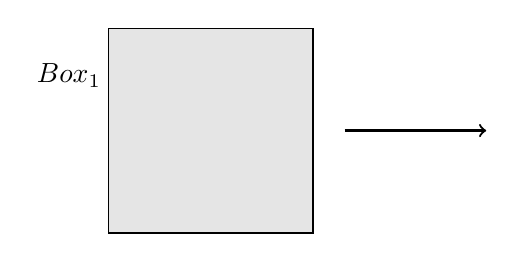
\begin{tikzpicture}
        % Set A
        \draw[fill=gray!20] (0,0) rectangle (2.6cm,2.6cm);
        \node at (-.5,2) {$Box_1$};

        % arrow
        \draw[->, thick] (3,1.3) -- (4.8,1.3);

    \end{tikzpicture}
    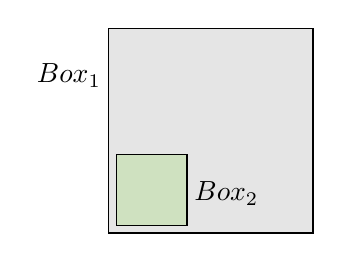
\begin{tikzpicture}
        % Set A
        \draw[fill=gray!20] (0,0) rectangle (2.6cm,2.6cm);
        \node at (-.5,2) {$Box_1$};

        % Set B
        \draw[fill=OliveGreen!20] (1,1) rectangle (.1cm,.1cm);
        \node at (1.5,0.5) {$Box_2$};

        \hfill
    \end{tikzpicture}
    \caption{\centering \underline{$Box_1$ contains \textbf{1} object,} which is $Box_2$ (an empty box). Hence $\quad$
        $Box_1$ represents $\{\{\}\}$ or $\{\emptyset\}$.}
    \label{fig:empty_box}
\end{figure}

\noindent
\underline{\textbf{$\emptyset$ is a subset of every set?}} Take sets $A=\{\}$ and $B=\{1,2,3\}$\\
By definition of a subset, every element in $A$ must be in $B$. It's difficult to
argue elements in $A$ are indeed in $B$, but it's undeniable that elements in $A$ are not in $B$.
Since our statement cannot be denied, it's \textbf{Vacuously true}.\\


\noindent
Counting the number of elements in a set is called the \textbf{cardinality} of the set.
\begin{theo}[Cardinality]{thm:cardinality}
    The number of elements in a set.\\
    Denoted over a set $A$ as $|A|$.
\end{theo}

\noindent
\textbf{For Example:}
\begin{itemize}
    \item $A = \{1, 2, 3\}$, $|A| = 3$.
    \item $B = \{a, e, i, o, u\}$, $|B| = 5$.
    \item $\mathbb{Z}$ the set of all integers, $|\mathbb{Z}| = \infty$.
\end{itemize}

\noindent
\textbf{Questions:}\\
What are the cardinalities of the following sets?
\begin{enumerate}
    \item $|\{1,2,3\}|$
    \item $|\emptyset|$
    \item $|\{\}|$
    \item $|\{\emptyset\}|$
    \item $|\{1,{2,3}\}|$
\end{enumerate}

\textbf{Answers:}
\begin{enumerate}
    \item 3
    \item 0
    \item 0
    \item 1
    \item 2
\end{enumerate}

\newpage

\noindent
Explicitly defining a set, say $\{1, 2, 3, ...\}$, is called \textbf{set-roster notation}.\\
\textbf{Set-builder notation} enables more complex definitions of a set.

\begin{theo}[Set-Builder Notation]{thm:set_builder}
    General form: $\{x \mid P(x)\}$,
    \begin{itemize}
        \item $x$ = defines some variable.
        \item $``\mid"$ = is short hand for ``such that.''
        \item $P(x)$ = describes the properties $x$ must satisfy.
    \end{itemize}
\end{theo}

\noindent
\textbf{For Example:} Lets define the set of even integers\\
\vspace{-1em}
\begin{itemize}
    \item $\{x \mid x \textnormal{ is an even integer}\}$: ``$x$, such that, $x$ is an even integer.''
    \item $\{x \in \mathbb{Z} \mid x \textnormal{ is even}\}$: ``$x$ in Integers, such that, $x$ is an even.''
    \item $\{x \in \mathbb{Z} \mid x \textnormal{ is not odd}\}$: ``$x$ in Integers, such that, $x$ is not odd.''
\end{itemize}

\noindent
\underline{\textbf{It's important to define exactly what variables are.}}
In the above, $x$ was stated directly as an integer. If not, x could be \underline{\textbf{water-balloons} or \textbf{puppies}.}

\subsection{Introduction to Sets}
\hspace*{1em}
In discrete math we work with some group of `things,' a thing or something
we fancily call an \textbf{object}. A group or categorization of objects is called a set.

\begin{theo}[Set]{thm:set}
    Is a collection of objects.
\end{theo}

\noindent
\textbf{For Example:}
\begin{itemize}
    \item $S$ = The set of all students in a classroom.
    \item $A$ = The set of all vowels in the English alphabet.
    \item $\mathbb{Z}$ = The set of all integers.

\end{itemize}
Objects in a \textbf{set} are called \textbf{elements}.

\begin{theo}[Element]{thm:element}
    An object that is a member of a given set.
\end{theo}

\noindent
To expand on the previous example:
\begin{itemize}
    \item $S = \{s_1, s_2, s_3\}$, where $s_1, s_2, s_3$ are students, elements of the set.
    \item $A = \{a, e, i, o, u\}$, where $a, e, i, o, u$ are elements.
    \item $\mathbb{Z} = \{\ldots, -3, -2, -1, 0, 1, 2, 3, \ldots\}$, elements of integer set.
\end{itemize}
Curly braces denote a set, commas separate elements, and
the `$...$' (ellipse) indicates an indefinite continuation, \underline{used only when the pattern \textbf{is clear.}}\\

\newpage

\noindent
There is also notation to denote members of a set.

\begin{theo}[Membership]{thm:membership}
    If $x$ is an element of set $A$, $x \in A$.
    If $x$ is not an element of set $A$, $x \notin A$.
\end{theo}

\noindent
\textbf{For Example:} Given $A = \{a, e, i, o, u\}$,\\
$a \in A$, ``$a$ is an element of $A$,'' and
$b \notin A$, ``$b$ is not an element of $A$.''\\

\noindent
\textbf{Order nor repetition matter:}
\begin{itemize}
    \item $A = \{1, 2, 3\} = \{3, 2, 1\} = \{1, 2, 3, 3, 3, 3, 3\}$.
    \item $B = \{a, b, c\} = \{a, b, c, a, b, c\}$.
\end{itemize}

\begin{theo}[Properties of a Set]{thm:set_props}
    \begin{itemize}
        \item The order of elements do not matter.
        \item Duplicate elements are not counted.
    \end{itemize}
\end{theo}


A subset is a set contained within another set. If the set $B$ is a subset of set $A$,
then every element in $B$ is also in $A$ as shown in Figure \ref{fig:subset}:


\begin{figure}[ht]
    \centering
    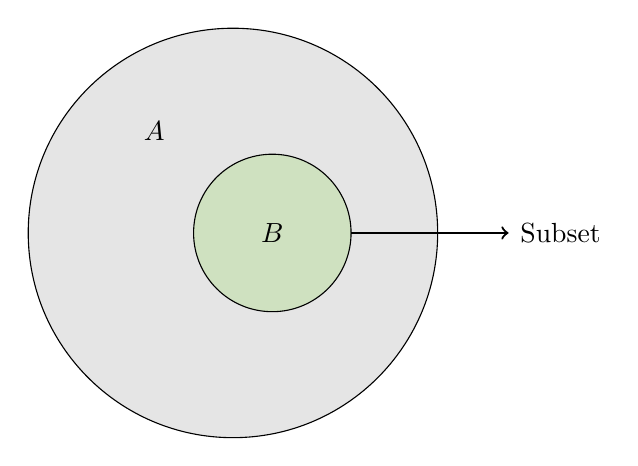
\begin{tikzpicture}
        % Set A
        \draw[fill=gray!20] (0,0) circle (2.6cm);
        \node at (-1,1.3) {$A$};

        % Set B
        \draw[fill=OliveGreen!20] (0.5,0) circle (1cm);
        \node at (0.5,0) {$B$};

        % Subset arrow
        \draw[->, thick] (1.5,0) -- (3.5,0);

        % Subset label
        \node at (4.16,0) {Subset};
    \end{tikzpicture}
    \caption{}
    \label{fig:subset}
\end{figure}


\noindent
Written $B \subseteq A$ or $A \supseteq B$, similar to the less than or
equal to signs `$\leq$' and `$\geq$'.

\newpage

\begin{theo}[Subset]{thm:subset}
    If every element in set $B$ is also in set $A$, then $B$ is a subset of $A$.\\
    Denoted: $B \subseteq A$ or $A \supseteq B$.
\end{theo}

\noindent
\textbf{For Example:}
\begin{itemize}
    \item $\{-1, 0\} \subseteq \{-1, 0, 1, 2, 3\}$
    \item $\{-1, 1, 3\} \subseteq \{-1, 0, 1, 2, 3\}$
    \item $\{-1, 0, 1, 2, 3\} \subseteq \{-1, 0, 1, 2, 3\}$
    \item $\{-1, 7\} \not\subseteq \{-1, 0, 1, 2, 3\}$
\end{itemize}

\underline{$\not\subseteq$ denotes `not a subset of.'}

\vspace{1em}

\noindent
A set with no elements is called the empty set.
\begin{theo}[Empty Set]{thm:empty_set}
    Commonly denoted by $\emptyset$ or $\{\}$, refers to a collection with no objects.
\end{theo}


\noindent
\textbf{Questions:}
\begin{enumerate}
    \item How many elements are in the set  $\{\emptyset\}$?
    \item True or False: $\emptyset \subseteq \{\emptyset\}$.
    \item True or False: $\emptyset \in \{\emptyset\}$.
    \item True or False: $\emptyset \subseteq \emptyset$.
    \item True or False: $\emptyset \subseteq \mathbb{Z}$.
    \item True or False: $\emptyset \in \mathbb{Z}$.
\end{enumerate}
\begin{Tip}
    Mathematicians define things? So can you! Let's define a collection that
    infinitely repeats the string ``bees.'' We will fancily call it\\
    ``\textbf{Bioths Non-determinant Sequence},'' or a $\beta_{seq}$ for short.
    $$\beta_{seq} = \{\textnormal{``bees''}, \textnormal{``bees''}, \textnormal{``bees''}, \textnormal{``bees''},
        \textnormal{``bees''}, \textnormal{``bees''}, \ldots\}$$

    \noindent
    \textbf{Names are names}, no matter how fancy, they were labeled
    by another human, like you. They thought,... ``Damn, this would be a \textit{kick-ass} name.''\\
    Never be intimidated, complex ideas are just groupings of basic concepts.
\end{Tip}
\newpage
\noindent
\textbf{Answers:}
\begin{enumerate}
    \item 1 element, the empty set.
    \item True, the empty set is a subset of $\{\emptyset\}$.
    \item True, the empty set is an element of $\{\emptyset\}$.
    \item True, the empty set is a subset of itself.
    \item True, the empty set is a subset of all sets.
    \item False, the empty set is not an element of the integers.
\end{enumerate}

\vspace{4em}

\noindent
\underline{\textbf{Why (1.):}} \textbf{A collection is an object}. The emptyset is a collection,
a collection without objects. Likewise, a house is still a house without furniture.\\

\noindent
\underline{\textbf{Why (5.):}} Take sets $A=\{\}$ and $B=\{1,2,3\}$\\
By definition of a subset, every element in $A$ must be in $B$. It's difficult to
argue elements in $A$ are indeed in $B$, but it's undeniable that elements in $A$ are not in $B$.
Since our statement cannot be denied, it's \textbf{Vacuously true}.\\

\noindent
\hrulefill\\

\noindent
Say we have an empty box. How many objects do we have? \textbf{Zero}.\\
Put an empty box inside our original box. How many objects now? \textbf{One}!


\begin{figure}[ht]
    $\hspace{.2cm}$
    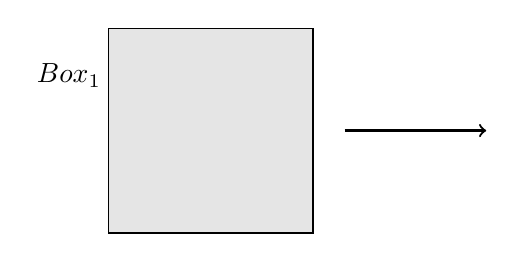
\begin{tikzpicture}
        % Set A
        \draw[fill=gray!20] (0,0) rectangle (2.6cm,2.6cm);
        \node at (-.5,2) {$Box_1$};

        % arrow
        \draw[->, thick] (3,1.3) -- (4.8,1.3);

    \end{tikzpicture}
    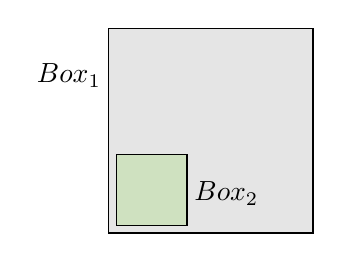
\begin{tikzpicture}
        % Set A
        \draw[fill=gray!20] (0,0) rectangle (2.6cm,2.6cm);
        \node at (-.5,2) {$Box_1$};

        % Set B
        \draw[fill=OliveGreen!20] (1,1) rectangle (.1cm,.1cm);
        \node at (1.5,0.5) {$Box_2$};

        \hfill
    \end{tikzpicture}
    \caption{\centering \underline{$Box_1$ contains 1 object,} which is $Box_2$, an empty box. Hence $\quad$
        $Box_1$ represents $\{\{\}\}$ or $\{\emptyset\}$.}
    \label{fig:empty_box}
\end{figure}

\noindent
\hrulefill\\

\newpage
\noindent
Counting the number of elements in a set is called the \textbf{cardinality} of the set.
\begin{theo}[Cardinality]{thm:cardinality}
    The number of elements in a set.\\
    Denoted over a set $A$ as $|A|$.
\end{theo}

\noindent
\textbf{For Example:}
\begin{itemize}
    \item $A = \{1, 2, 3\}$, $|A| = 3$.
    \item $B = \{a, e, i, o, u\}$, $|B| = 5$.
    \item $\mathbb{Z}$ the set of all integers, $|\mathbb{Z}| = \infty$.
\end{itemize}

\noindent
\textbf{Questions:}\\
What are the cardinalities of the following sets?
\begin{enumerate}
    \item $|\{1,2,3\}|$
    \item $|\emptyset|$
    \item $|\{\}|$
    \item $|\{\emptyset\}|$
    \item $|\{1,\{2,3\}\}|$
    \item $|\{1,2,2,3,3,3\}|$
\end{enumerate}

\vspace{1em}

\noindent
\textbf{Try to think about the answer before looking at the solution.}\\
Things stick when you struggle.\\

\begin{Tip}
    Whenever you approach a problem, always break things down into simple components.
    ``What defines a set? What defines an element? What defines a subset? What defines cardinality?''\\
\end{Tip}

\noindent
\textbf{Answers:}
\begin{enumerate}
    \item 3
    \item 0
    \item 0
    \item 1
    \item 2
    \item 3
\end{enumerate}

\newpage

\noindent
Explicitly defining a set, say $\{1, 2, 3, ...\}$, is called \textbf{set-roster notation}.\\
\textbf{set-builder notation} enables us to create more complex definitions.

\begin{theo}[Set-Builder Notation]{thm:set_builder}
    General form: $\{x \mid P(x)\}$,
    \begin{itemize}
        \item $x$ = defines some variable.
        \item $``\mid"$ = is short hand for ``such that.''
        \item $P(x)$ = describes the properties $x$ must satisfy.
    \end{itemize}
\end{theo}

\noindent
\textbf{For Example:} Lets define the set of even integers\\
\vspace{-1em}
\begin{itemize}
    \item $\{x \mid x \textnormal{ is an even integer}\}$: ``$x$, such that, $x$ is an even integer.''
    \item $\{x \in \mathbb{Z} \mid x \textnormal{ is even}\}$: ``$x$ in Integers, such that, $x$ is an even.''
    \item $\{x \in \mathbb{Z} \mid x \textnormal{ is not odd}\}$: ``$x$ in Integers, such that, $x$ is not odd.''
\end{itemize}

\noindent
\underline{\textbf{It's important to define exactly what variables are.}}
In the above, $x$ was stated directly as an integer. If not, x could be \underline{\textbf{water-balloons} or \textbf{puppies}.}

\subsection{Set Operations}

% Subraction

Combining the two sets, $\{1,2,3\}$ and $\{a,b,c\}$, produce the set $\{1,2,3,a,b,c\}$, which
is called the \textbf{union}.\\

\begin{Def}[Union]{def:union}
    The set of elements that appear in either set $A$ or set $B$ is the union.\\
    Denoted: $A \cup B$.
\end{Def}

\noindent
This is also known as a \textbf{disjunction}, which is a fancy term for the word ``OR".\\

\noindent
\textbf{For Example:}
\begin{itemize}
    \item $\{1, 2\} \cup \{2, 3\} = \{1, 2, 3\}$.
    \item $\{1,2\} \cup \emptyset = \{1, 2\}$. There is nothing to add.
    \item $\{1\} \cup \{\emptyset\} = \{1, \emptyset\}$. The $\emptyset$ is an element in this case.
\end{itemize}

\newpage
\noindent
The common elements of the two sets, $\{1,2,3\}$ and $\{2,3,4\}$, produce the set $\{2,3\}$,
the \textbf{intersection}.\\

\begin{Def}[Intersection]{def:intersection}
    The set of elements that appear in both sets $A$ and $B$ is the intersection.\\
    Denoted: $A \cap B$.
\end{Def}

\noindent
This is also known as a \textbf{conjunction}, which is a fancy term for the word ``AND".\\

\noindent
\textbf{For Example:}
\begin{itemize}
    \item $\{1, 2\} \cap \{2, 3\} = \{2\}$.
    \item $\{1\} \cap \{2\} = \emptyset$. There is nothing in common.
    \item $\{1\} \cap \emptyset = \emptyset$. There is nothing to compare.
\end{itemize}

\begin{Tip}
    To lessen the confusion between $\cup$ and $\cap$, think, ``$\cap$" for ``AND",\\
    since $\cap$ looks like a curved ``A" without the line. \\
\end{Tip}

\noindent
The combination of $A=\{1,2,3\}$ and $B=\{a,b,c\}$ in order pairs are:
$$(1,a), (1,b), (1,c), $$
$$(2,a), (2,b), (2,c), $$
$$(3,a), (3,b), (3,c)$$

\noindent
Putting the above objects in a set yields the \textbf{cartesian product} of $A$ and $B$.

\begin{Def}[Cartesian Product]{def:cartesian}
    The set of all possible order pairs of elements from sets $A$ and $B$.\\
    Denoted: $A \times B$.
\end{Def}

\noindent
\textbf{For Example:}
\begin{itemize}
    \item $\{1, 2\} \times \{a, b\} = \{(1,a), (1,b), (2,a), (2,b)\}$.
    \item $\{1,2\} \times \emptyset = \emptyset$. There is nothing to pair.
    \item $\{1\} \times \{\emptyset\} = \{(1,\emptyset)\}$. The $\emptyset$ is an element in this case.
\end{itemize}

\begin{Note}
    \textbf{Note:} Visit `\textbf{Figure \ref{fig:empty_box}}' in the previous section if $\emptyset$ causes confusion.
\end{Note}


\noindent
We have sets $A=\{1,2,3\}$ and $B=\{2,3,4\}$, to remove the common elements
$A$ has with $B$, i.e., take all in $A$ that is not in $B$, yields the set $\{1\}$, the \textbf{difference}.\\

\begin{Def}[Difference]{def:difference}
    The set of all elements that are in set $A$ but not in set $B$.\\
    Denoted: $A - B$.
\end{Def}

\noindent
\textbf{For Example:}
\begin{itemize}
    \item $\{1, 2\} - \{2, 3\} = \{1\}$.
    \item $\{1\} - \{1\} = \emptyset$.
    \item $\{1,2\} - \emptyset = \{1, 2\}$. There is nothing to remove.
\end{itemize}

\noindent
All possible subsets of a set is called the \textbf{power set}.
\begin{Def}[Power Set]{def:power}
    The set of all subsets of a set.\\
    Denoted: $\mathcal{P}(A)$, $A$ is a set.
\end{Def}

\noindent
\textbf{For Example:}
\begin{itemize}
    \item $\mathcal{P}(\emptyset) = \{\emptyset\}$.
    \item $\mathcal{P}(\{1\}) = \{\emptyset, \{1\}\}$.
    \item $\mathcal{P}(\{1, 2\}) = \{\emptyset, \{1\}, \{2\}, \{1, 2\}\}$.
    \item $\mathcal{P}(\{1, 2, 3\}) = \{\emptyset, \{1\}, \{2\}, \{3\}, \{1, 2\}, \{1, 3\}, \{2, 3\}, \{1, 2, 3\}\}$.
\end{itemize}

\noindent
The number of subsets grow exponentially with the number of elements in the set.
The rate it grows is $2^{|n|}$, where $n$ is the number of elements in the set.

\begin{Def}[Power Set Cardinality]{def:pow_set_card}
    The cardinality of the power set grows $2^{|n|}$, where $n$ is the number of elements in the set.
\end{Def}

\newpage

\noindent
There are more operations that we could discuss, but we will stop here for now.
I encourage you challenge these definitions create different cases, and test them.\\

\begin{greenbox}
    \textbf{Summary:} A \textbf{set} is a collection of `things' or objects. An object that is a member of a set is an
    \textbf{element} $4\in\mathbb{Z}$. In a set \textbf{order and
        repetition do not matter}. Sets can contain other sets, these subsections/slices/portions are
    called \textbf{subsets}. An \textbf{empty set} is denoted $\emptyset$ or $\{\}$. \textbf{Cardinality} is the element
    count of a set, it does not count sets beyond the top layer. $\{1, {2, 3}\}$ has a cardinality of 2, not 3.
    \textbf{Set-roster} notation is the explicit listing of a set like $\{...,1,2,3,...\}$. \textbf{Set-builder}
    notation is the description of a set $\{x\in \mathbb{Z} | x \textbf{ is even}\}$. Combining two sets is called a \textbf{union},
    the \textbf{intersection} is the common elements between two sets. The \textbf{cartesian product} of two sets is the set of all possible
    ordered pairs. The \textbf{difference} between sets $A$ and $B$ are elements in $A$ that are not in $B$. There
    are many more operations that we could discuss, but we will just stick to these for now.
\end{greenbox}

\begin{graybox}
    \textbf{Comments:} In or out of math, we talk about sets. In conversations,\\
    ``yeah that thing!" ``sorry, what thing?"
    Those people: are we talking about the group or a sub-group of those people. Will we make generalizations?
    Will we be specific? To draw connections, Humans $\in$
    Earth $\in$ Universe. Organizing files, sub-folder to sub-folder. Everything is a set of something.
\end{graybox}
\vspace{1em}

\newpage
\section{Functions}
\subsection{Introduction to Functions}
To talk about functions, is to talk about \textbf{relationships}. Take the `<' sign, this
is a relationship. $x < y$ means $x$ relates to $y$, such that $x$ is less than $y$.\\

\noindent
\begin{center}
    Let $a=\{1,2,3,4\}$, $b=\{0,1,2,3\}$. Let $R$ be the relation `<', $aRb$ yields:
\end{center}

\vspace{1em}
\begin{figure}[ht]
    \centering
    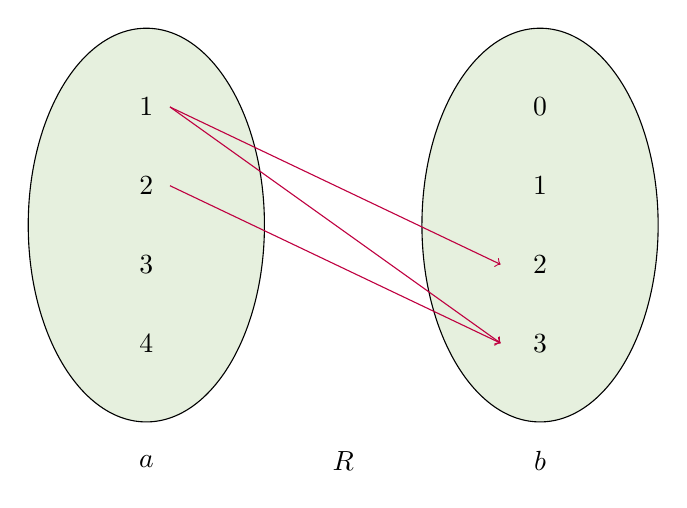
\begin{tikzpicture}
        % Draw the sets
        \draw[black, fill=OliveGreen!10] (-3,0) ellipse (1.5 and 2.5);
        \draw[black, fill=OliveGreen!10] (2,0) ellipse (1.5 and 2.5);


        % Labels for the elements in the first set
        \node at (-3,1.5) {1};
        \node at (-3,.5) {2};
        \node at (-3,-.5) {3};
        \node at (-3,-1.5) {4};
        \node at (-3,-3) {$a$};

        % Labels for the elements in the second set
        \node at (2,1.5) {0};
        \node at (2,.5) {1};
        \node at (2,-.5) {2};
        \node at (2,-1.5) {3};
        \node at (2,-3) {$b$};

        \node at (-.5,-3) {$R$};

        % Draw the arrow
        %1
        \draw[->, purple] (-2.7,1.5) -- (1.5,-.5);
        \draw[->, purple] (-2.7,1.5) -- (1.5,-1.5);

        %2
        \draw[->, purple] (-2.7,.5) -- (1.5,-1.5);
    \end{tikzpicture}
    \caption{\centering $R$ produces ordered pairs $\{(1,2),(1,3),(2,3)\}$, as $1<2$, $1<3$, $2<3$}.
    \label{fig:relates}
\end{figure}

\begin{Def}[Relation]{thm:relation}
    A relation $R$ on sets $a$ and $b$, $aRb$, is a subset of $a\times b$.
\end{Def}

\noindent
Since $a\times b$ is the set of all possible ordered pairs. $R$'s pairings must contain some or
all pairing of $a\times b$. This includes no pairing at all, the emptyset.\\

\noindent
The arrows in \textbf{Figure \ref{fig:relates}} are often referred to as \underline{\textbf{mappings}}. 1 maps to 2, 1 maps to 3, and 2 maps to 3.\\

\begin{Tip}
    When looking at Definitions, come up with examples on your own. The ability to explain a concept to someone else
    proves understanding.\\
\end{Tip}

\newpage


\begin{figure}
    Functions are a type of relation, where \underline{\textbf{each input has exactly one output.}}\\
    We can visualize this as a machine:\\\\


    \hspace{3em}
    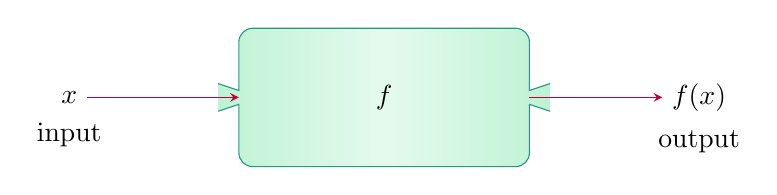
\begin{tikzpicture}
        \node[label={below:{input}}] (A) at (3,0) {$x$};
        \pic (B) at (7,0) {machine={$f$}};
        \node[label={below:{output}}] (C) at (11,0) {$f(x)$};

        \draw[purple, -stealth] (A) -- (B-in);
        \draw[purple, -stealth] (B-out) -- (C);

    \end{tikzpicture}
    \caption{\centering The machine $f$ takes an input $x$ and produces an output $f(x)$.}
    \label{fig:machine}
\end{figure}

\noindent
In our previous example we used `<' as a relation. This is not a function, as\\
$1$ relates to $2$ and $3$. Instead let's use the absolute function, $f(x)=|x|$.

\begin{figure}[ht]
    \centering
    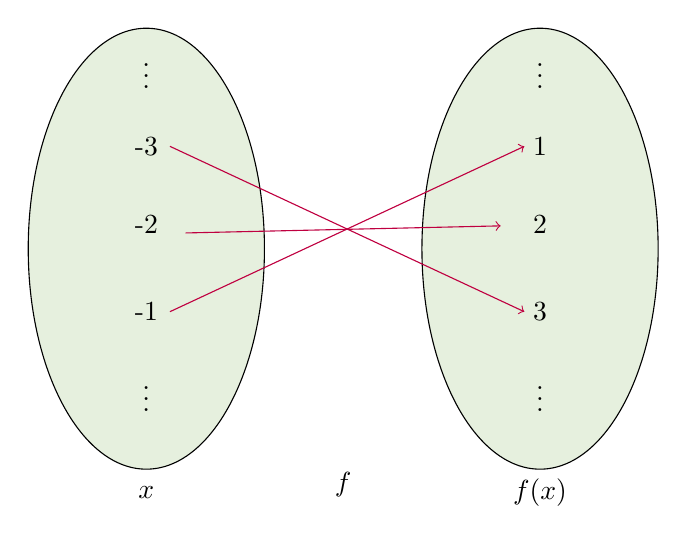
\begin{tikzpicture}
        % Draw the sets
        \draw[black, fill=OliveGreen!10] (-3,0) ellipse (1.5 and 2.8);
        \draw[black, fill=OliveGreen!10] (2,0) ellipse (1.5 and 2.8);


        % Labels for the elements in the first set
        \node at (-3,2.3) {\vdots};
        \node at (-3,1.3) {-3};
        \node at (-3,.3) {-2};
        \node at (-3,-.8) {-1};
        \node at (-3,-1.8) {\vdots};
        \node at (-3,-3.1) {$x$};

        % Labels for the elements in the second set
        \node at (2,2.3) {\vdots};
        \node at (2,1.3) {1};
        \node at (2,.3) {2};
        \node at (2,-.8) {3};
        \node at (2,-1.8) {\vdots};
        \node at (2,-3.1) {$f(x)$};

        \node at (-.5,-3) {$f$};

        % Draw the arrow
        %-3
        \draw[->, purple] (-2.7,1.3) -- (1.8,-.8);
        %-2
        \draw[->, purple] (-2.5,.2) -- (1.5,.29);
        %-1
        \draw[->, purple] (-2.7,-.8) -- (1.8,1.3);
    \end{tikzpicture}
    \caption{\centering Pairs $\{(-3,3),(-2,2),(-1,1)\}$, as $f(-3)=3$, $f(-2)=2$, $f(-1)=1$}.
    \label{fig:relates}
\end{figure}

\begin{Note}
    \textbf{Note}: f(x)=|x| is where x hasn't been chosen yet, choose 3, f(-3)=|-3|=3.
\end{Note}

\noindent
In \textbf{Figure \ref{fig:relates}}, assume inputs are integers. Then the absolute functions maps to \\
integers, i.e., \underline{if I put in an integer, I get out an integer.} In the figure we\\
represent this by the two green ovals; The left (inputs), the right (outputs).\\

\noindent
Our inputs are called the \textbf{domain}, the outputs the \textbf{codomain},\\
and all the possible mappings the \textbf{range}.\\

\newpage

\begin{Def}[Function]{Def:function}
    A function $f$ is a relation between two sets, $A$ (the domain) and $B$ (the codomain),
    such that each element in $A$ is mapped to exactly one element
    in $B$. The set of all possible outputs of $f$ is called the range of $f$.
\end{Def}

\noindent
Say we create a function $f(x)$, which tells us if someone prefers cats or dogs.\\

\begin{center}
    Let $P=\{\text{``Lois"}, \text{``Pete"}, \text{``Stuart"}\}$, $Q=\{\text{"Cats"}, \text{"Dogs"}\}$.
\end{center}

\begin{figure}[ht]
    \centering
    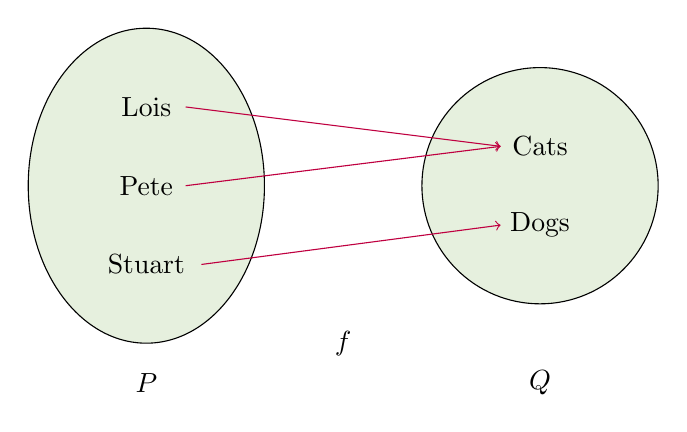
\begin{tikzpicture}
        % Draw the sets
        \draw[black, fill=OliveGreen!10] (-3,0) ellipse (1.5 and 2);
        \draw[black, fill=OliveGreen!10] (2,0) ellipse (1.5 and 1.5);


        % Labels for the elements in the first set
        \node at (-3,1) {Lois};
        \node at (-3,0) {Pete};
        \node at (-3,-1) {Stuart};
        \node at (-3,-2.5) {$P$};

        % Labels for the elements in the second set
        \node at (2,.5) {Cats};
        \node at (2,-.5) {Dogs};
        \node at (2,-2.5) {$Q$};

        \node at (-.5,-2) {$f$};

        % Draw the arrow
        %Lowis
        \draw[->, purple] (-2.5,1) -- (1.5,.5);
        %Peter
        \draw[->, purple] (-2.5,0) -- (1.5,.5);
        %Stewie
        \draw[->, purple] (-2.3,.-1) -- (1.5,-.5);
    \end{tikzpicture}
    \caption{\centering Produced ordered pairs $\{(\text{Lois},\text{Cats}),(\text{Pete},\text{Cats}),(\text{Stuart},\text{Dogs})\}$.}
    \label{fig:cats_dogs}
\end{figure}

\noindent
In function $f$, \underline{all elements in our domain map to an element in our
    codomain.} This makes our function \textbf{onto}, or \textbf{surjective}.\\

\begin{Def}[Onto (Surjective)]{thm:onto}
    A function $f$ is onto if every element in the codomain is mapped to by some element in the domain.
\end{Def}

\newpage

\noindent
Now say we have a function $g(x)$, which tells us a person's student ID.\\
\begin{center}
    Let $T=\{\text{``Raven"}, \text{``Stella"}, \text{``Robbert"}\}$, $U=\{\text{"U001"}, \text{"U002"}, \text{U003}, ...\}$.
\end{center}

\begin{figure}[ht]
    \centering
    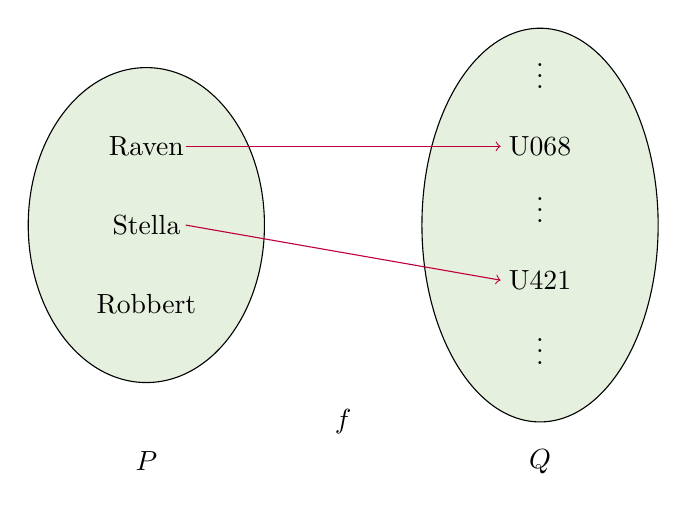
\begin{tikzpicture}
        % Draw the sets
        \draw[black, fill=OliveGreen!10] (-3,0) ellipse (1.5 and 2);
        \draw[black, fill=OliveGreen!10] (2,0) ellipse (1.5 and 2.5);


        % Labels for the elements in the first set
        \node at (-3,1) {Raven};
        \node at (-3,0) {Stella};
        \node at (-3,-1) {Robbert};
        \node at (-3,-3) {$P$};

        % Labels for the elements in the second set
        \node at (2, 2) {\vdots};
        \node at (2, 1) {U068};
        \node at (2,.3) {\vdots};
        \node at (2,-.7) {U421};
        \node at (2,-1.5) {\vdots};
        \node at (2,-3) {$Q$};

        \node at (-.5,-2.5) {$f$};

        % Draw the arrow
        %Raven
        \draw[->, purple] (-2.5,1) -- (1.5,1);
        %Stella
        \draw[->, purple] (-2.5,0) -- (1.5,-.7);
    \end{tikzpicture}
    \caption{\centering Produced ordered pairs $\{(\text{Raven},\text{U068}),(\text{Stella},\text{U421})\}$.
        not all elements have a mapping, meaning it is \textbf{not onto}.}
    \label{fig:cats_dogs}
\end{figure}

\noindent
In our example this suggests that ``Robbert" is not a registered student.\\

\noindent
\underline{Each element in the domain maps to exactly one element in the codomain.}\\
This makes our function \textbf{one-to-one}, or \textbf{injective}.\\

\begin{Def}[One-to-One (Injective)]{thm:one_to_one}
    A function $f$ is one-to-one if each element in the domain is mapped to exactly one element in the codomain.
\end{Def}

\begin{Tip}
    To remember the difference between `surjective' and `injective': think, one-to-one,
    one-to-one means a personal connection, something unique, one goes \textbf{into} one, \textbf{`i'}
    for \textbf{`into'}, \textbf{`i'} for \textbf{`injective'}.\\

\end{Tip}

\newpage

\noindent
If we were to change the function $g$, restricting the domain to only include
registered students, then our function would be \textbf{onto} and \textbf{one-to-one}. Since
each student has a unique ID, and each ID belongs to a student.\\

\noindent
When a function is both onto and one-to-one, it is called a \textbf{bijection}.\\

\begin{Def}[Bijection]{thm:bijection}
    A function $f$ is a bijection if it is both onto and one-to-one.
\end{Def}
\vspace{2em}
\begin{greenbox}
    \begin{spacing}{1.5}
        \textbf{Summary: } A \textbf{function} is a \textbf{relationship} between two sets. A set for which we use
        as an input, and a set that will house our outputs. A relationship can be described in
        ordered pairs, take sets $A$ and $B$, over some relation $R$, $x\in A$ relates to $y\in B$
        such that $(x,y)\in R$. The ordered pairs in a \underline{relation is a subset of $A\times B$},
        which includes the emptyset.\\

        \noindent
        A function takes in one input and produces one output. The set of all our inputs is called the
        \textbf{domain}, the set of our outputs the \textbf{codomain}. The set of all possible mappings
        from the domain to the codomain is called the \textbf{range}.\\

        \noindent
        If elements in the codomain all have a mapping, the function is \textbf{onto} or\\
        \textbf{surjective}. If elements in the codomain have a unique mapping, the function is
        \textbf{one-to-one} or \textbf{injective}.
        If a function is both \textbf{onto} and \textbf{one-to-one}, it is \textbf{bijective}.
    \end{spacing}
\end{greenbox}


\newpage

\section{Logic}
\subsection{Introduction to Logic}
\vspace{1em}
Observe the claim below:
\vspace{1em}
\begin{center}
    \Large
    \textit{``You're a rotten cook and your breath is sickly."}
\end{center}
\vspace{1em}

\noindent
This \textbf{assertion} is a \textbf{statement} or \textbf{proposition} that is either \underline{\textbf{TRUE} or \textbf{FALSE}}.\\

\vspace{-1em}
\begin{Note}
    \textbf{Note:} claim, assertion, statement, and proposition are all synonyms.
\end{Note}

\vspace{1em}
\noindent
\textbf{Most Importantly:}
\begin{itemize}
    \item Am I actually a rotten cook?
    \item Is my breath really that sickly?
\end{itemize}

\noindent
We can boil down these two propositions to the following:
\begin{itemize}
    \item $R$: You're a rotten cook
    \item $S$: Your breath is sickly
\end{itemize}

\vspace{1em}
\noindent
The original claim can be rewritten as:
\begin{itemize}
    \item ``$R$ and $S$'' formally written, ``$R \land S$'', ``$\land$'' shorthand for ``AND.''\\
          \underline{\textbf{Both} proposition must be true} for the claim to be true.
\end{itemize}

\vspace{1em}
\noindent
Altering the claim to \textit{``You're a rotten cook or your breath is sickly''} yields:
\begin{itemize}
    \item ``$R$ or $S$'' formally written, ``$R \lor S$'', ``$\lor$'' shorthand for ``OR.''\\
          \underline{\textbf{At least one} of the proposition must me true} for the claim to be true.\\\\
          ``\textit{Maybe you're a rotten cook, maybe your breath is sickly, maybe both}.''
\end{itemize}

\begin{Tip}
    To remember the difference between ``$\land$'' and ``$\lor$'', think: $\land$ looks like an ``A''
    without the line for ``AND''.\\

    \noindent
    Also remember ``And'' is CONJUNCTION, ``OR'' is DISJUNCTION. To
    help, think conjunction means ``conjoin'' to join together,\\ ``I'm putting together
    one and one, I'm \textit{conjoining} them.''\\
\end{Tip}

\noindent
Observe the claim below:
\vspace{1em}
\begin{center}
    \Large
    \textit{``I'm not a rotten cook, but I admit my breath is sickly."}
\end{center}
\vspace{1em}

\noindent
The above states, ``Not $R$'' formally written, ``$\neg R$'', ``$\neg$'' shorthand for ``NOT''.
\underline{``but'' in this context is a conjunction.} The claim writes as: ``$\neg R \land S$''.\\

\begin{Tip}
    Try to uncover what a statement is truly saying, not literally.
    In language we often obfuscate sentences to hide intent or to be more polite.\\
\end{Tip}

\noindent
Observe the claim below:
\vspace{1em}
\begin{center}
    \Large
    \textit{``Either I'm a rotten cook or my breath is sickly,\\ not both."}
\end{center}
\vspace{1em}

\noindent
This is an example of the \textbf{exclusive OR} (XOR), we'll use the symbol ``$\oplus$''.\\
Written as ``$R \oplus S$'', \underline{\textbf{only one} of the proposition can be true, not both.}\\

\noindent
This is more obvious in statements such as:
\begin{itemize}
    \item ``They either went to the party or stayed home.''
    \item ``You are either with me or against me.''
    \item ``They either bought lunch or saved their money.''
\end{itemize}

\noindent
We call ``$\land, \lor, \neg, \oplus$'', \textbf{logical operators}.

\begin{Def}[Logical Operators]{def:logical}
    A symbol that represents a logical operation.
    \begin{itemize}
        \item $\land$: AND, both must be true.
        \item $\lor$: OR, at least one must be true.
        \item $\neg$: NOT, negation, opposite.
        \item $\oplus$: XOR, exclusive OR, either or, but not both.
    \end{itemize}
\end{Def}

\newpage

\noindent
\subsection{Statements vs. Predicates:}
Below reads, \underline{\textbf{``4 is less than 2.''} This is false}, but still \textbf{is a statement}:
\begin{center}
    \large
    $4<2$
\end{center}
A statement evaluates to either true or false, \textbf{predicates don't}. Such as:
\begin{center}
    \large
    $x<2$
\end{center}
\textbf{This is a predicate}, it's neither true or false until we assign a value to $x$.\\

\begin{Def}[Proposition]{def:proposition}
    A statement that is either true or false, independent of any variables.
\end{Def}
\begin{Def}[Predicate]{def:predicate}
    A statement where its truth values depend on one or more variables.
\end{Def}


\Div

\subsection{Truth Tables}
Writing whole sentences in logic can be cumbersome even in their reduced logical forms.
So we use \textbf{truth tables} to help keep track our evaluations.\\

\noindent
To demonstrate, let's use a table to show the values $P$ and $\neg P$\\
Our goal is to \underline{find all possible values} of $P$ to then evaluate $\neg P$.\\
Let's take that concept and evaluate $P$ and $Q$ for ``$P \land Q$'' and ``$P \lor Q$.''\\

\begin{center}
    \begin{tabular}{|c|c|}
        \hline
        \rowcolor{OliveGreen!10}
        $P$ & $\neg P$ \\
        \hline
        T   & F        \\
        F   & T        \\
        \hline
    \end{tabular}
\end{center}
\noindent
$T$ = ``True'' and $F$ = ``False'', we refer to these truth values as \underline{\textbf{booleans}}.\\


\begin{Def}[Boolean]{def:boolean}
    A Boolean is a value that can only be either true or false.
\end{Def}

\newpage

\noindent
Our goal here is to find all possible value combinations of $P$ and $Q$ to then evaluate $P \land Q$ and $P \lor Q$.\\


\begin{center}
    \begin{tabular}{|c|c|c|c|}
        \hline
        \rowcolor{OliveGreen!10}
        $P$ & $Q$ & $P \land Q$ & $P \lor Q$ \\
        \hline
        T   & T   & T           & T          \\
        T   & F   & F           & T          \\
        F   & T   & F           & T          \\
        F   & F   & F           & F          \\
        \hline
    \end{tabular}
\end{center}

We will read this table's $P$ then $Q$ boolean values respectively:
\begin{enumerate}
    \item $T$ then $T$, So $T\land T = T$, and $T\lor T = T$.
    \item $T$ then $F$, So $T\land F = F$, and $T\lor F = T$.
    \item $F$ then $T$, So $F\land T = F$, and $F\lor T = T$.
    \item $F$ then $F$, So $F\land F = F$, and $F\lor F = F$.
\end{enumerate}

\begin{Tip}
    When working with new concepts, ask yourself what was going through the creator's mind.
    Try to understand the logic and intuition behind concepts rather than memorizing them.
    So when you forget, you'll be able to derive the concept from scratch, or consider a new novel idea.\\
\end{Tip}
\Div


\subsection{Boolean Algebra}

In digital systems we manipulate binary values to evaluate logic. These systems use
states of \underline{``on'' and ``off'' to represent 1 (true) and 0 (false).}\\

\noindent
This is identical to the propositional logic we've been discussing. Observe:\\
\begin{center}
    \begin{tabular}{c c c}
        Boolean Algebra &     & Propositional Logic \\
        \hline
        $\bar{x}$       & NOT & $\neg x$            \\
        $x \cdot y$     & AND & $x \land y$         \\
        $x + y$         & OR  & $x \lor y$          \\
        $x \oplus y$    & XOR & $x \oplus y$        \\
        \hline
    \end{tabular}
\end{center}

\begin{Note}
    \textbf{Note:} XOR in programming is often represented by the caret symbol `$^\wedge $'.
\end{Note}

\noindent
This is the basis for logic gates and circuits, of which we will not discuss here.\\

\newpage

\noindent
Lets use the following truth table to demonstrate boolean algebra conversion:\\
\begin{center}
    \begin{tabular}{|c|c|c|}
        \hline
        \rowcolor{OliveGreen!10}
        $P$ & $Q$ & $f(x)$ \\
        \hline
        T   & T   & F      \\
        T   & F   & T      \\
        F   & T   & F      \\
        F   & F   & T      \\
        \hline
    \end{tabular}
\end{center}

\begin{tabular}{cc|l}
    \textbf{DNF}                                  & \textbf{CNF}                                 &                     \\
    \hline
    $(P \land \neg Q) \lor (\neg P \land \neg Q)$ & $(\neg P \lor \neg Q) \land (P \lor \neg Q)$ & Propositional Logic \\
    $(P \cdot \bar{Q}) + (\bar{P} \cdot \bar{Q})$ & $(\bar{P} + \bar{Q}) \cdot (P + \bar{Q})$    & Boolean Algebra     \\
    \hline
\end{tabular}

\vspace*{2em}

\noindent
We say \underline{$(P\bar{Q}) + (\bar{P} \bar{Q})$ is \textbf{equivalent} to $(\bar{P} + \bar{Q}) (P + \bar{Q})$.}
This doesn't mean they are syntactically the same or re-arrangeable to match. Rather that they evaluate to the same truth values.\\

\noindent
I.e, we could swap out $f(x)$ for either of the two expressions and \underline{the truth table remains the same.}\\

\begin{Note}
    \textbf{Note:} the dot refers to multiplication so ``$P\cdot Q$'' is ``$PQ$'', they are one and the same.
\end{Note}

\begin{Def}[Logical Equivalence]{def:log_equiv}
    Two expressions are equivalent if they evaluate to the same truth values.\\
    Denoted: $P \equiv Q$.
\end{Def}

\noindent
Obverse the claim:
\begin{center}
    \Large
    \textit{``If you don't study, then you won't pass.''}
\end{center}

This is an example of a \textbf{conditional statement}. Let's break the statement down:
\begin{itemize}
    \item \textbf{S} to study.
    \item \textbf{P} to pass.
\end{itemize}

\noindent
The statement says, ``$\neg S$ \textbf{implies} $\neg P$'', i.e.,
``$\neg S$ \textbf{then} $\neg P$'', formally written as ``$\neg S \rightarrow \neg P$.''\\

\newpage

\noindent
This type of statement is called an \textbf{implication}.
\begin{Def}[Implication]{def:imp}
    A conditionally statement of the form, if $P$ then $Q$.\\
    Denoted: $P \rightarrow Q$.
\end{Def}

\noindent
Observe the following truth table for the implication:

\begin{center}
    \begin{tabular}{|c|c|c|}
        \hline
        \rowcolor{OliveGreen!10}
        $P$ & $Q$ & $P \rightarrow Q$ \\
        \hline
        T   & T   & T                 \\
        T   & F   & F                 \\
        F   & T   & T                 \\
        F   & F   & T                 \\
        \hline
    \end{tabular}
\end{center}

\noindent
Think of the implication as holding a promise:
\begin{itemize}
    \item If the promise to do something, and it gets done, I held my promise (true).
    \item If I promise to do something, and it doesn't get done, I broke my promise (false).
    \item If I never promised to do anything, then I can't break my promise (true).
\end{itemize}
The last statement is true because \underline{there was no promise to break,} hence, it's \textbf{Vacuously True}.\\
Likewise, you cannot deny my claim if I never made one.\\

\begin{Note}
    \textbf{Note:} We say a \textbf{vacuously true} statement before when saying $\emptyset$ is a subset of all sets.
    As it's impossible to deny that nothing is a part of something.
\end{Note}

\noindent


\noindent
Before we learned about Demorgan's Laws, and Double Negation. We'll need a couple more laws
to help us further understand and manipulate these forms.\\

\noindent
Reference the below table of logical equivalences, (This will be your best friend):\\

\noindent
\begin{tabular}{|p{2cm}|l|l|}
    \hline
    Idempotent:                  & $p\lor p\equiv p$                                   & $p\land p\equiv p$                                   \\
    \hline
    Associative:                 & $(p\lor q) \lor r \equiv p \lor (q \lor r)$         &
    $(p\land q) \land r \equiv p \land (q\land r)$                                                                                            \\
    \hline
    Commutative:                 & $p\lor q\equiv q \lor p$                            & $p\land q \equiv q \land p$                          \\
    \hline
    Distributive:                & $p\lor (q\land r) \equiv (p\lor q) \land (p\lor r)$ & $p\land (q\lor r) \equiv (p\land q) \lor (p\land r)$ \\
    \hline
    Identity:                    & $p\lor F \equiv p$                                  & $p\land T\equiv p$                                   \\
    \hline
    Domination:                  & $p\land F \equiv F$                                 & $p\lor T\equiv T$                                    \\
    \hline
    Double Negation:             & \multicolumn{2}{l|}{$\neg\neg p\equiv p$}                                                                  \\
    \hline
    \multirow{2}{*}{Complement:} & $p\land \neg p \equiv F$                            & $p\lor \neg p \equiv T$                              \\
                                 & $\neg T \equiv F$                                   & $\neg F \equiv T$                                    \\
    \hline
    De Morgan's Laws:            & $\neg(p\lor q) \equiv \neg p \land \neg q$          &
    $\neg(p\land q) \equiv \neg p \lor \neg q$
    \\
    \hline
    Absorption:                  & $p\lor (p\land q) \equiv p $                        & $p\land (p\lor q) \equiv p$                          \\
    \hline
    Conditional identities:      & $p\rightarrow q \equiv \neg p \lor q$               &
    $p\leftrightarrow q \equiv (p\rightarrow q)\land (q\rightarrow p)$                                                                        \\
    \hline
\end{tabular}

\newpage



\noindent
\textbf{Questions:}\\
Of the following, which is DNF and which is CNF, or both?

\begin{enumerate}
    \item $P\land Q\lor \neg W$
\end{enumerate}

\Div

\subsection{Set equivalences}

\noindent
The same way we say, ``it will rain today'' is a proposition, so is,\\
``a set $S$ has an element $x$.'' Using this knowledge we can apply logical equivalences.\\

\noindent
Observe the statement, ``$A=\{1,2\}$ and $B=\{3,4\}$; $A \cap B$.'' Breaking it down:
\begin{itemize}
    \item $A \cap B$ means $x\in A \land y\in B$.
    \item $x\in A$ means $x$ equals ``1 or 2.''
    \item $y\in B$ means $y$ equals ``3 or 4.''
\end{itemize}

\noindent
Describing ``$A \cap B$'' in terms of ``$x\in A \land y\in B$'' allows us to manipulate the expression.\\

\newpage

\noindent
Just like we had equivalence laws for propositions, we have equivalence laws for sets.\\

\noindent
{\Large \textbf{Set Equivalences:}\\}

\noindent
\begin{tabular}{|p{2cm}|l|l|}
    \hline
    \cellcolor{OliveGreen!10} Idempotent:                                            & $A\cup A= A$                                                    & $A\cap A= A$                                 \\
    \hline
    \cellcolor{OliveGreen!10} Associative:                                           & $(A\cup B) \cup C = A \cup (B \cup C)$                          &
    $(A\cap B) \cap C = A \cap (B\cap C)$                                                                                                                                                             \\
    \hline
    \cellcolor{OliveGreen!10} Commutative:                                           & $A\cup B= B \cup A$                                             & $A\cap B = B \cap A$                         \\
    \hline
    \cellcolor{OliveGreen!10} Distributive:                                          & $A\cup (B\cap C) = (A\cup B) \cap (A\cup C)$                    & $A\cap (B\cup C) = (A\cap B) \cup (A\cap C)$ \\
    \hline
    \cellcolor{OliveGreen!10} Identity:                                              & $A\cup \O = A$                                                  & $A\cap U= A$                                 \\
    \hline
    \cellcolor{OliveGreen!10} Domination:                                            & $A\cap \O = \O$                                                 & $A\cup U=A$                                  \\
    \hline
    \cellcolor{OliveGreen!10} Double Negation:                                       & \multicolumn{2}{l|}{$\overline{\overline{A}}=A$}                                                               \\
    \hline
    \cellcolor{OliveGreen!10}\multirow{2}{*}                                         & $A\cap \overline{A} = \O$                                       & $A\cup \overline{A} = U$                     \\
    \cellcolor{OliveGreen!10}\raisebox{.8\normalbaselineskip}[0pt][0pt]{Complement:} & $\overline{U} = \O$                                             & $\overline{\O} = U$                          \\
    \hline
    \cellcolor{OliveGreen!10} De Morgan's Laws:                                      & $\overline{A\cup B} =  \overline{A} \cup \overline{B}$          &
    $\overline{A\cap B} = \overline{A} \cup \overline{B}$
    \\
    \hline
    \cellcolor{OliveGreen!10} Absorption:                                            & $A\cup (A\cap B) = A $                                          & $A\cap (A\cup B) = A$                        \\
    \hline
    \cellcolor{OliveGreen!10} Subset:                                                & \multicolumn{2}{l|}{$A\subseteq B = x\in A \rightarrow x\in B$}                                                \\
    \hline
    \cellcolor{OliveGreen!10} Union:                                                 & \multicolumn{2}{l|}{$A\cap B = x\in A \land x\in B$}                                                           \\
    \hline
    \cellcolor{OliveGreen!10} Intersection:                                          & \multicolumn{2}{l|}{$A\cup B = x\in A \lor x\in B$}                                                            \\
    \hline
\end{tabular}

\vspace{1em}

\noindent
\textbf{For Example:}

\textit{\textbf{Prove:} $A\cup (B\cap C) = (A\cup B) \cap (A\cup C)$.}

\begin{center}
    \begin{tabular}{l l m{.1mm} l m{.1mm} l l}
        1. & $A$ & $\cup$ & $ (B\cap C) $ &  &  & \text{Given} \\
        1. & $A$ & $\cup$ & $ (B\cap C) $ &  &  & \text{Given} \\
    \end{tabular}
\end{center}
\Div

\subsection{Set Quantifiers}
Set quantifiers help describe particular members of a set. Let's examine \underline{the set of
    all musical artists.}\\

\noindent
Observe the claim:

\begin{center}
    \Large
    \textit{``Artists that live in texas, make country music."}
\end{center}

\noindent
This claim generalizes an entire group of artist. Perhaps not all
Texan artists make country music. This is called a {\textbf{universal generalization}}.\\

\noindent
Using Set-Builder notation:
\begin{itemize}
    \item $A$, is the set of all artists.
    \item $T(x)$, returns true if $x$ is from Texas.
    \item $C(x)$, returns true if $x$ makes country music.
    \item Yielding, ``for all $x\in A \mid T(x) \rightarrow C(x)$.''
    \item Reads, \underline{``for all $x$ in $A$, if $x$ is from Texas, then $x$ makes country music.''}
\end{itemize}

\noindent
The symbol for \underline{``For All'' is ``$\forall$''}, an upside-down ``A'', which gives us:

\begin{center}
    \Large
    ``$\forall x \in A \mid T(x) \rightarrow C(x)$.''
\end{center}

\newpage

\begin{Def}[Universal Generalization]{def:universal}
    A claim that applies to all elements in a set.
    Denoted: $\forall x \in A \mid P(x) \rightarrow Q(x)$, given a set $A$ and predicates $P(x)$ and $Q(x)$.
\end{Def}

\noindent
Observe the claim:

\begin{center}
    \Large
    \textit{``There exists an artist that lives in Texas, that makes dubstep."}
\end{center}

\noindent
Here we describe a particular artist. This is called an {\textbf{existential instantiation}}.\\

\noindent
Using Set-Builder notation:
\begin{itemize}
    \item $A$, is the set of all artists.
    \item $T(x)$, returns true if $x$ is from Texas.
    \item $D(x)$, returns true if $x$ makes dubstep.
    \item Yielding, ``there exists an $x\in A \mid T(x) \land D(x)$.''
    \item Reads, \underline{``there exists an $x$ in $A$, such that $x$ is from Texas and makes dubstep.''}
\end{itemize}

\noindent
The symbol for \underline{``There Exists'' is ``$\exists$''}, an backwards ``E'', which gives us:

\begin{center}
    \Large
    ``$\exists x \in A \mid T(x) \land D(x)$.''\\
\end{center}

\begin{Def}[Existential Instantiation]{def:existential}
    A claim that applies to at least one element in a set.\\
    Denoted: $\exists x \in A \mid P(x) \land Q(x)$, given a set $A$ and predicates $P(x)$ and $Q(x)$.
\end{Def}

\noindent
An existential claim creates the set of all elements that satisfy the claim. So there \textit{could}
exist multiple artists that live in Texas and make dubstep.

\noindent
\subsection*{When to use $\rightarrow$ vs. $\land$:}
\begin{itemize}
    \item \textbf{Universal Generalization:} Uses ``$\rightarrow$'' to imply a relationship.
    \item \textbf{Existential Instantiation:} Uses ``$\land$'' to describe qualities of a particular member.
\end{itemize}

\newpage

\subsection{Nested Quantifiers}

\noindent
Consider the claim:

\begin{center}
    \Large
    \textit{``Every artist in a record label, has someone else as their manager."}
\end{center}

\begin{itemize}
    \item $P$, the set of all people.
    \item $A(x)$, $x$ is an artist.
    \item $R(x)$, $x$ has a record label.
    \item $M(x, y)$, $y$ is $x$'s manager.
\end{itemize}

\noindent
We are dealing with two predicates, someone who is $x$ and someone who is $y$. Breaking it down:
\begin{itemize}
    \item $E$ = Every artist in a record label = $\forall x \in P \mid A(x) \land R(x)$.
    \item $S$ = Said artist has a manager =  $\exists y \in P \mid M(x, y)$.
    \item $E$ implies $S$, so $E \rightarrow S$.
    \item Yielding, \underline{$(\forall x \in P \mid A(x) \land R(x)) \rightarrow (\exists y \in P \mid M(x, y))$.}
\end{itemize}

\noindent
Our final statement reads:

\begin{center}
    \Large
    ``For all $x$ in $P$, if $x$ is an artist and has a record label, then there exists a $y$ in $P$ that is $x$'s manager.''
\end{center}

\noindent
Or concisely:\\

\begin{center}
    \Large
    ``For every x there exists y in P, if x is an artist and has a record label, then y is x's manager.''
\end{center}

\noindent
Written:\\

\begin{center}
    \Large
    $\forall x \exists y \in P \mid (A(x)\land R(x)) \rightarrow M(x,y)$
\end{center}

\noindent
If the set is clear, we can omit syntax and write:\\

\begin{center}
    \Large
    $\forall x \exists y \enspace (A(x)\land R(x)) \rightarrow M(x,y)$
\end{center}

% Quantifiers with sets -
% Negating quantifiers
% show manipulating sets with boolean alg -
% equivalence relations
% show functional completeness
% series and sequences
% proofs
% modular arithmetic

\end{document}
